\chapter{Background} \label{chap:Background}

\label{chap:background}
	\textit{In this chapter, we introduce the foundation knowledge of the thesis, including the history and definition of Blockchain Technology, Cryptocurrency, 
	Hierarchical Deterministic Wallet (HD Wallet) and Cryptography}
\minitoc

\section{Blockchain Technology}

\subsection{History and Definition}

Blockchains are immutable digital ledger systems implemented in a distributed fashion (i.e., without a central repository) and usually without a central authority.
The definition of blockchain was introduced to the world by a person (or a group of people) under the name Satoshi Nakamoto on October 31, 2008. 
It was applied to enable the emergence of a "purely peer-to-peer (no financial institution or third party) electronic cash" named Bitcoin where transactions take place in a distributed system.
In fact, Satoshi did not invent blockchain, and Bitcoin blockchain is not the first chain that ever created. 
Back in 1991, cryptographers Stuart Haber and Scott Stornetta published a whitepaper "How to Time-Stamp a Digital Document" in the Journal of Cryptography. 
Their goal is to digital time-stamping of documents so that it is infeasible for a user either to back-date or to a forward-date digital document, even with the collusion of a time-stamping service. 
The technology is called a blockchain because the distributed electronic ledger stores items of data in time-stamped digital groups called blocks. Each block includes an alphanumeric code called a "hash" summing up its data. The hash of each completed block also appears in the next one in the chain, which means that to alter one block you would have to alter all the ones connected to it. These cryptographic dominos function together to protect against tampering or fraud.
Base on this theory, the longest-running blockchain, started in 1995, also by Haber and Stornetta, publishes the weekly summary hash value every week in the New York Times (\autoref{fig:first_blockchain}) and still running strong today. 

\begin{figure}[h!]
	\centering
	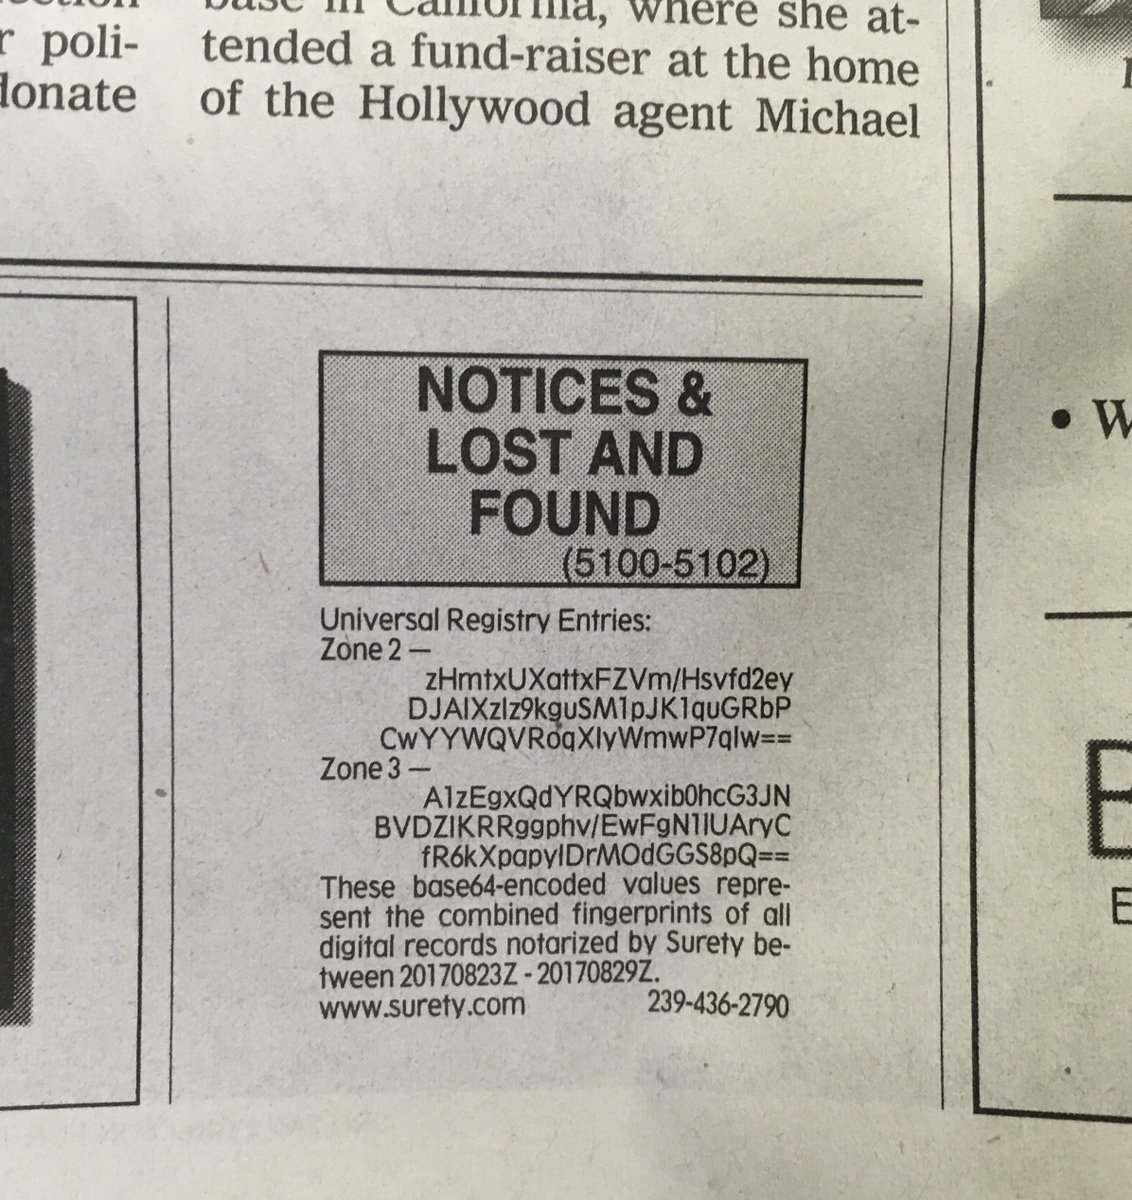
\includegraphics[width=.35\textwidth]{images/Widely_Witnessed_Values.jpg}
	\caption[Widely-Witnessed Values of Surety, a weekly summary (hash) of documents]{Weekly summary hash value in The New York Times}
	\label{fig:first_blockchain}
\end{figure}

The math behind blockchain and its complex system architecture make it challenging to understand. 
NIST provided an informal concise description of blockchain technology:

\begin{quote} 
Blockchains are distributed digital ledgers of cryptographically signed transactions that are grouped into blocks. 
Each block is cryptographically linked to the previous one after validation and undergoing a consensus decision. 
As new blocks are added, older blocks become more difficult to modify. 
New blocks are replicated across all copies of the ledger within the network, and any conflicts are resolved automatically using established rules. 
\end{quote}

Blockchain technology comes handy in a wide range of areas - both ​financial​ and non-financial​. 
Non-Financial​ application opportunities are endless. 
We can envision putting proof of the existence of all legal documents, health records, and loyalty payments in the music industry, notary, private securities and marriage licenses in the blockchain. 
By storing the fingerprint of the digital asset instead of storing the digital asset itself, the anonymity or privacy objective can be achieved.
For the sake of our thesis, we will mainly focus on the original and surely the most popular application of blockchains - Cryptocurrency.

Cryptocurrencies are digital currencies that use blockchain technology to record and secure every transaction. 
A cryptocurrency can be used as a digital form of cash that can be used to buy goods and services. 
It can be bought using one of several digital wallets or trading platforms, then digitally transferred upon purchase of an item, with the blockchain recording the transaction and the new owner. 
The appeal of cryptocurrencies is that everything is recorded in a public ledger and secured using cryptography, making an irrefutable, timestamped, and secure record of every payment.
The ledger displays user account balances and inter-user payments in a “currency” defined by the ledger itself and not necessarily in one of the traditional currencies. 
Nevertheless, cryptocurrency may be traded on the stock exchange and exchanged for traditional money, which makes it hard to distinguish between traditional currency and cryptocurrency and as official vs. non-official currency. 
The most widely recognized cryptocurrency system is Bitcoin.

We believe the "magic" that brings the above concept of digital cash to reality, besides blockchain technology, is Nakamoto's proof-of-work consensus model.

\subsection{Bitcoin blockchain architecture}
Bitcoin is the first application of blockchain and also a very successful practice
As mentioned above, Bitcoin was invented with the publication of a document entitled "Bitcoin: A peer-to-peer electronic cash system" in 2008 by Satoshi Nakamoto, mentioned as a purely P2P version of electronic cash would allow online payments to be sent directly from one party to another without going through a financial institution.
And for the first time in the history of distributed computing

Its system is composed of the storage layer and the network layer of the protocol layer, including all kinds of scripts, 
1and the intelligent contract extension layer, which encapsulates the application layer of all kinds of applications. 

All levels coordinate with each other to maintain the stability of the system 





\section{HD Wallet}



\subsection{Category}

\subsection{Coins}

\subsection{Wallet structure}

\section{Cryptography}

\subsection{Cryptographic hash}

\subsection{Diffie-Hellman algorithm}

\subsection{RSA}

\subsection{ECC}

\subsubsection{Blockchain: secp256k1}

\subsubsection{Discrete logarithm problem}

\subsection{Twisted-Edward curve and Ed25519}

\subsection{Key derivation function}
